\begin{verbatim}


 [V, n, p, res, niter] = secs1d_nlpoisson_newton (x, sinodes, Vin, nin, pin,
                                                  Fnin, Fpin, D, l2, er, toll, maxit)

     input:  
             x       spatial grid
             sinodes index of the nodes of the grid which are in the semiconductor subdomain
                     (remaining nodes are assumed to be in the oxide subdomain)
             Vin     initial guess for the electrostatic potential
             nin     initial guess for electron concentration
             pin     initial guess for hole concentration
             Fnin    initial guess for electron Fermi potential
             Fpin    initial guess for hole Fermi potential
             D       doping profile
             l2      scaled Debye length squared
             er      relative electric permittivity
             toll    tolerance for convergence test
             maxit   maximum number of Newton iterations

     output: 
             V       electrostatic potential
             n       electron concentration
             p       hole concentration
             res     residual norm at each step
             niter   number of Newton iterations


\end{verbatim}




\subsection{Demo 1 for function secs1d\_nlpoisson\_newton}
\begin{verbatim}

 secs1d_physical_constants
 secs1d_silicon_material_properties
 
 tbulk= 1.5e-6;
 tox = 90e-9;
 L = tbulk + tox;
 cox = esio2/tox;
 
 Nx  = 50;
 Nel = Nx - 1;
 
 x = linspace (0, L, Nx)';
 sinodes = find (x <= tbulk);
 xsi = x(sinodes);
 
 Nsi = length (sinodes);
 Nox = Nx - Nsi;
 
 NelSi   = Nsi - 1;
 NelSiO2 = Nox - 1;
 
 Na = 1e22;
 D = - Na * ones (size (xsi));
 p = Na * ones (size (xsi));
 n = (ni^2) ./ p;
 Fn = Fp = zeros (size (xsi));
 Vg = -10;
 Nv = 80;
 for ii = 1:Nv
     Vg = Vg + 0.2;
     vvect(ii) = Vg; 
     
     V = - Phims + Vg * ones (size (x));
     V(sinodes) = Fn + Vth * log (n/ni);
     
     % Scaling
     xs  = L;
     ns  = norm (D, inf);
     Din = D / ns;
     Vs  = Vth;
     xin   = x / xs;
     nin   = n / ns;
     pin   = p / ns;
     Vin   = V / Vs;
     Fnin  = (Fn - Vs * log (ni / ns)) / Vs;
     Fpin  = (Fp + Vs * log (ni / ns)) / Vs;
     
     er    = esio2r * ones(Nel, 1);
     l2(1:NelSi) = esi;
     l2    = (Vs*e0)/(q*ns*xs^2);
     
     % Solution of Nonlinear Poisson equation
     
     % Algorithm parameters
     toll  = 1e-10;
     maxit = 1000;
     
     [V, nout, pout, res, niter] = secs1d_nlpoisson_newton (xin, sinodes, 
                                                            Vin, nin, pin,
                                                            Fnin, Fpin, Din, l2,
                                                            er, toll, maxit);
 
     % Descaling
     n     = nout*ns;
     p     = pout*ns;
     V     = V*Vs;
     
     qtot(ii) = q * trapz (xsi, p + D - n);
 end
 
 vvectm = (vvect(2:end)+vvect(1:end-1))/2;
 C = - diff (qtot) ./ diff (vvect);
 plot(vvectm, C)
 xlabel('Vg [V]')
 ylabel('C [Farad]')
 title('C-V curve')
\end{verbatim}

\begin{figure}\centering
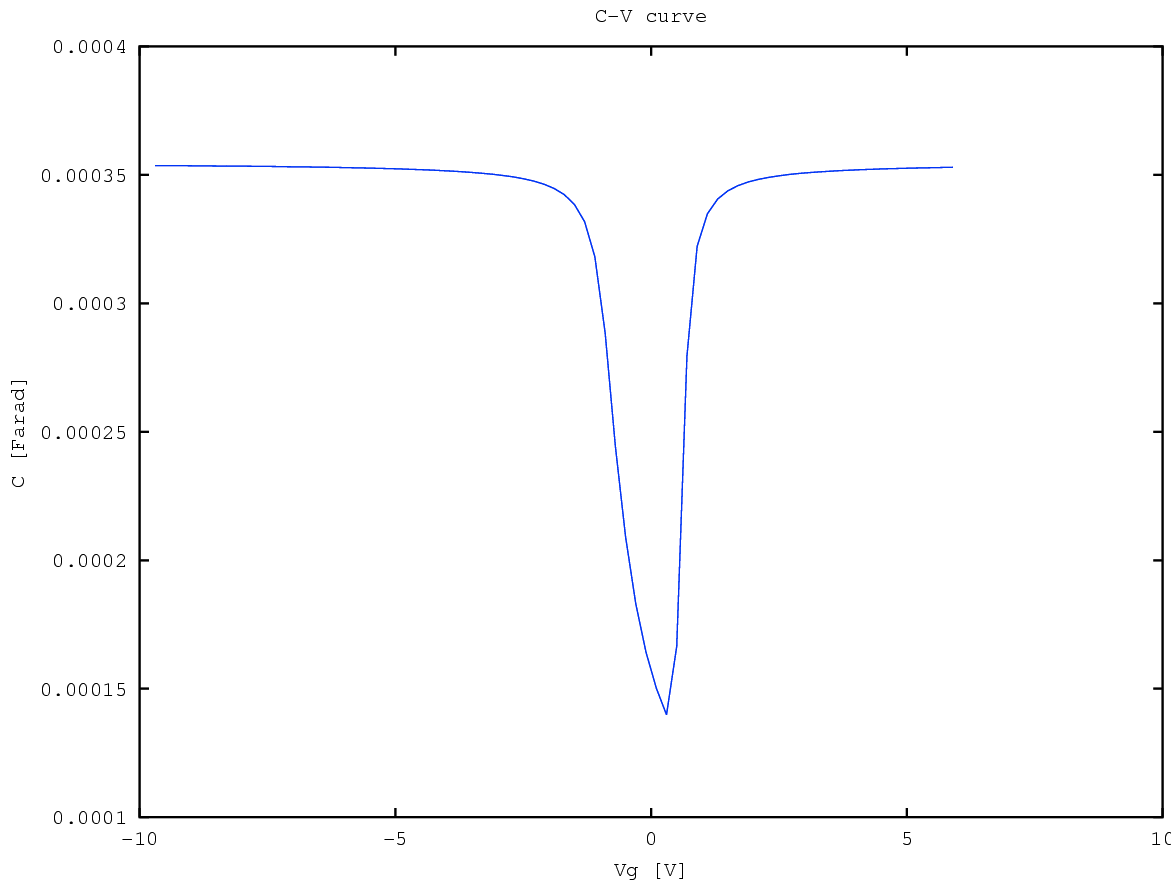
\includegraphics[width=.7\linewidth]{function/images/secs1d_nlpoisson_newton_85.png}
\caption{Figure produced by demo number 1 for function secs1d\_nlpoisson\_newton}
\label{fig:secs1d_nlpoisson_newton_figure_1}
\end{figure}
\clearpage
